\section{Results}\label{sec:fusana}

Discrete auroral drivers can be broadly divided into quasi-static inverted-V structures and Alfvén waves (AW).
AW-driven auroral forms include splitting auroral arcs and flaming aurora.
Discrete auroral arcs driven by sources other than dispersive Alfvén waves include kinked auroral arcs and non-flaming, non-splitting discrete arcs.
HiST can distinguish between the differential number flux precipitation signatures responsible for AW and non-AW aurora.

Inverted-V potential drops have several associated mechanisms that can lead to fast time-dependent behavior such an intensity modulation.
Inverted-V auroral features do not have dispersive energy behaviors associated with them--precipitating particles across a range of energies arrive at roughly the same time $\Delta t \ll \unit[10]{ms}$ difference.
Double layers, and series of double layers may exist within an inverted-V structure giving rise to narrower width auroral arcs.

AW are associated with reconfiguration of the magnetosphere--particularly during the breakup and expansion phase of substorms, where a quarter-trillion watts are launched towards Earth \citep{mottez2015}.
AW are integral to the settling out of the system after a change in current flux.
The conditions favorable for DAW aurora are delineated in Figure~\ref{fig:alfvenblock}.
\begin{figure}\centering 
    %the \par is necessary after each text to make the \baselineskip take effect
    \begin{tikzpicture}[node distance=1.5cm, auto]
    
    \node (magdis) [startstop,text width=4cm] {Magnetospheric discontinuity (e.g. reconnection) \par };
       
    \node (iaw) [process, below of = magdis,xshift=-1 cm] {IAW $B_\parallel$ \par };
    
    \node (kaw) [process,right of = iaw,xshift=1 cm] {KAW $B_\parallel$ \par };
    
    \node (wl) [decision, below of=iaw,text width=2 cm,yshift=-0.75cm] { cold plasma  $\omega < \omega_{ci}$ $v_A > v_{te}$ \par };
    
    
    \node (iontherm) [estimate, below of=wl,yshift=-1 cm, text width=5cm]{ $k \sim$ ion thermal gyroradius: $ \rho_i = \frac{\sqrt{T_i/m_i}}{\omega_{ci}} $ \par};
    
    \node (iongyro) [estimate, left of=iontherm,xshift=-4cm, text width=4cm]{ $k \sim$ ion gyroradius: $ \rho_s = \frac{\sqrt{T_e/m_i}}{\omega_{ci}} $ \par};
    
    \node (eskin) [estimate, right of=iontherm,xshift=4cm,text width=4cm]{ $k \sim$ electron skin depth: $\lambda_e = \frac{c}{\omega_{pe}}$ \par};
    
    \node (accel) [process, below of=iontherm,yshift=-0.25cm]{$ E_\parallel$ \par};
    
    \node(eflux) [process,below of=accel,text width=4cm]{100x background dispersive or flat-top electron flux $\Phi$ \par};
    
    \node(lt) [startstop, below of=eflux,xshift=-2cm]{Langmuir Turbulence \par};
    
    \node(aurora) [startstop, below of=eflux,xshift=2cm]{Alfvénic Aurora \par};
    
    \node(neial) [compute,below of=lt,xshift=-1cm] {NEIALs \par};
    \node(isr) [compute,below of=neial]{ISR backscatter \par};
    \node(isrest)[startstop,below of=isr,text width=3cm,yshift=-.5cm]{CFAR Turbulence estimate \par};
    
    \node(hist)[compute,below of=aurora,xshift=1cm]{HiST: filter, camera};
    \node(det)[compute,below of=hist,text width=3cm,yshift=-.5cm]{HiST: Alfvénic discrimination algorithm};
    \node(est)[startstop,below of=det,text width=3cm,yshift=-.75cm]{HiST: $\Phi_{top}$ precipitation estimation};
    
    \draw[arrow] (magdis) -- (iaw);
    \draw[arrow] (magdis) -- (kaw);
    \draw[arrow] (iaw) -- (wl);
    \draw[arrow] (wl) -- (iongyro);
    \draw[arrow] (wl) -- (iontherm);
    \draw[arrow] (wl) -- (eskin);
    \draw[arrow] (iongyro) -- (accel);
    \draw[arrow] (iontherm) -- (accel);
    \draw[arrow] (eskin) -- (accel);
    \draw[arrow] (accel) -- (eflux);
    \draw[arrow] (eflux) -- (aurora);
    \draw[arrow] (eflux) -- (lt);
    
    \draw[arrow] (lt) -- (neial);
    \draw[arrow] (neial) -- (isr);
    \draw[arrow] (isr) -- (isrest);
    
    \draw[arrow] (aurora) -- (hist);
    \draw[arrow] (hist) -- (det);
    \draw[arrow] (det) -- (est);
    
    \end{tikzpicture}
    \caption{Block diagram of Alfvénic aurora acceleration mechanism and HiST observation.}
    \label{fig:alfvenblock}
\end{figure}
A key ground-observable characteristic of Alfvénic aurora is narrow arc width.
``Width'' describes spatial scale size in the dimension perpendicular to geomagnetic field $B$.
\citet{maggsdavis1968} noted that the lower observed limit of \unit[70]{m} arc width was instrumentally limited.
\citet{borovsky1993} noted that observations from contemporary ground-based auroral arc measurements continued to reveal arc widths less than \unit[100]{m}.
Alfvénic aurora are associated with a sudden large increase in flux of particles accelerated from a few eV to as much as \unit[10]{keV} \citep{chaston2003}.
Due to dispersion along the accelerated particle path, over several hundred milliseconds \citep{dahlgren2013} the characteristic energy $E_0$ will go from order \unit[10]{keV} to order \unit[100]{eV}.
A representative differential number flux for a DAW event is shown in Figure~\ref{fig:alfvenflux}.
\begin{figure}
    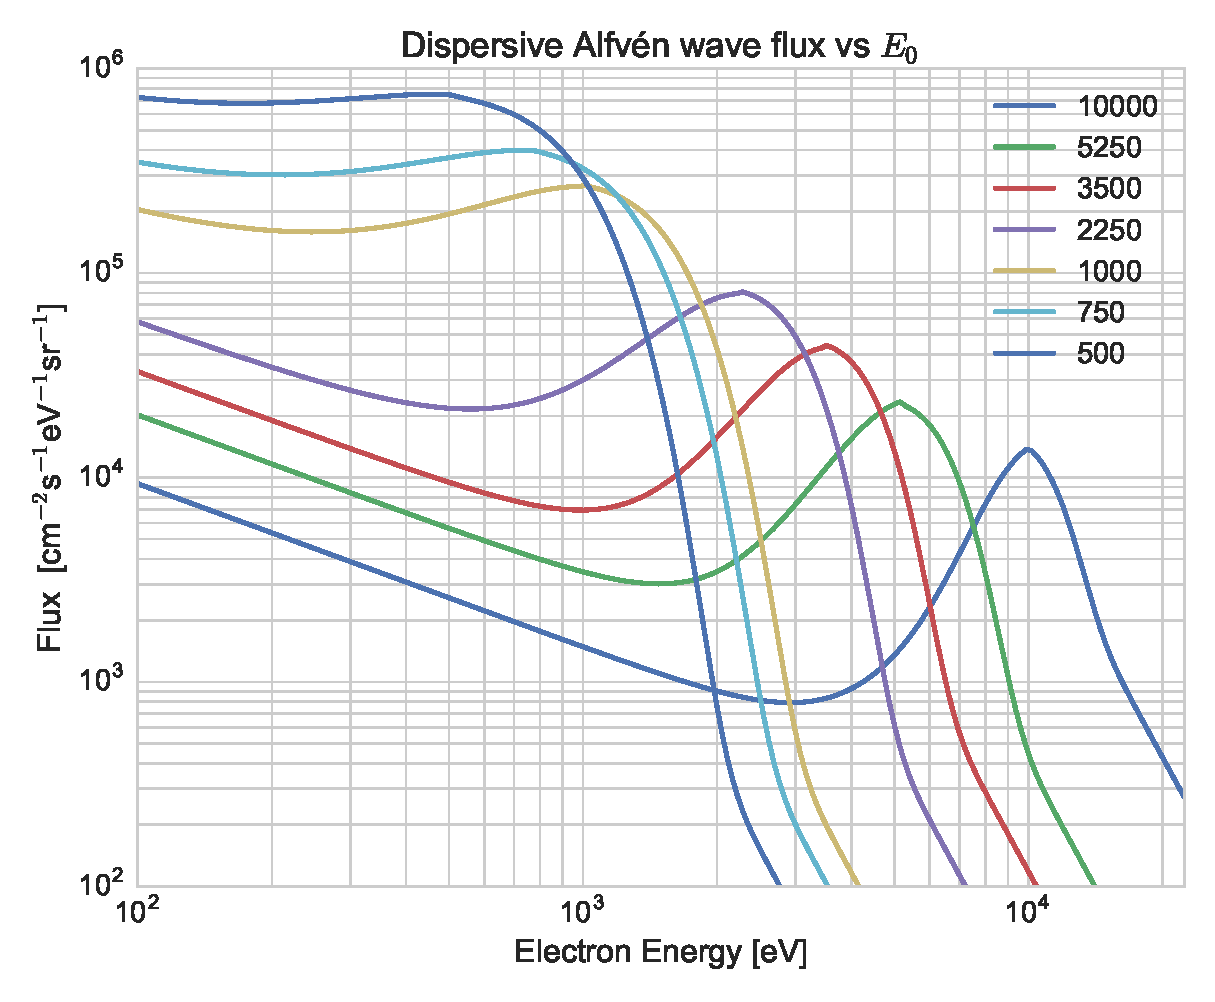
\includegraphics[width=0.9\columnwidth]{gfx/eflux}
    \caption{Evolution of characteristic energy $E_0$ from order \unit[10]{keV} to order \unit[100]{eV} occurs in \unit[100..1000]{ms} for DAW.
    In this plot, overall flux $Q_0$ is held constant.}
    \label{fig:alfvenflux}
\end{figure}
\textit{In situ} Freja measurements with \unit[32]{kHz} sampling rate \citep{stasiewicz2000} consistently showed plasma evacuations by roughly a factor of two near magnetic perturbations along $B_\parallel$ consistent with the presence of Alfvén waves.
Considering the \unit[7]{km/s} platform motion, the spectrograms of magnetic field point to $k_\perp \in [10,7000]$~m.
Freja also observed clear correlations \citep{stasiewicz2000} with turbulent magnetic field and suprathermal electron bursts ranging from \unit[100]{eV} to \unit[20]{keV} with particle fluxes of order 100 times over the background, and Poynting flux of $\unit[1..20]{mW/m^2}$.

The sampling cadence configuration of PFISR and the optical instruments for each experiment is given in Table~\ref{tab:cadence}.
These raw sample times are far faster than the minute cadence typically employed for plasma parameter estimation, yet those minute-long estimates break down in the face of these transient events.
We examine four types of events in turn: auroral breakup, splitting auroral arc, flaming auroral arc, and kinked arc with joint analysis of optical, spectral and radar features.


\FloatBarrier
\subsection{Breakup Auroral Arcs}\label{sec:breakup}
Highly dynamic events may combine several auroral morphologies, driven by diverse acceleration mechanisms, yielding multiple plasma turbulence types in close spatiotemporal proximity.
These events are difficult to interpret with instruments smearing in time by a factor of 100..1000 times greater than the ground-observable timescales.
It is also impractical to have a human manually initiating recording during extended observations.
This fact motivates the automatic Alfvénic aurora discrimination algorithms cited in section~\ref{sec:hist}.

A canonical example of such an event motivating the HiST system was the auroral breakup of March 23, 2007 shown in Figure~\ref{fig:20070323}.
\begin{figure}
    \noindent\includegraphics[width=0.9\columnwidth,trim=0 383 0 10,clip]{gfx/2007-03-23/2007-03-23}
    \vspace{0.1cm}
    
    % psd ion-line
    \includegraphics[width=0.3\columnwidth,trim=0 55 0 0]{gfx/2007-03-23/acfslice_alternatingcode2007-03-2311-20-08}
    \includegraphics[width=0.3\columnwidth,trim=0 55 0 0]{gfx/2007-03-23/acfslice_alternatingcode2007-03-2311-20-23}
    \includegraphics[width=0.3\columnwidth,trim=0 55 0 0]{gfx/2007-03-23/acfslice_alternatingcode2007-03-2311-20-39}
    
    \vspace{-0.5cm}
    \hspace{0.1cm}(f)\hspace{0.275\columnwidth}(g)\hspace{0.275\columnwidth}(h)
    \vspace{0.1cm}
    
    % psd plasma-line
    \includegraphics[width=0.45\columnwidth,trim=0 60 0 0]{gfx/2007-03-23/plasmaDOWNslice2007-03-2311-20-08}
    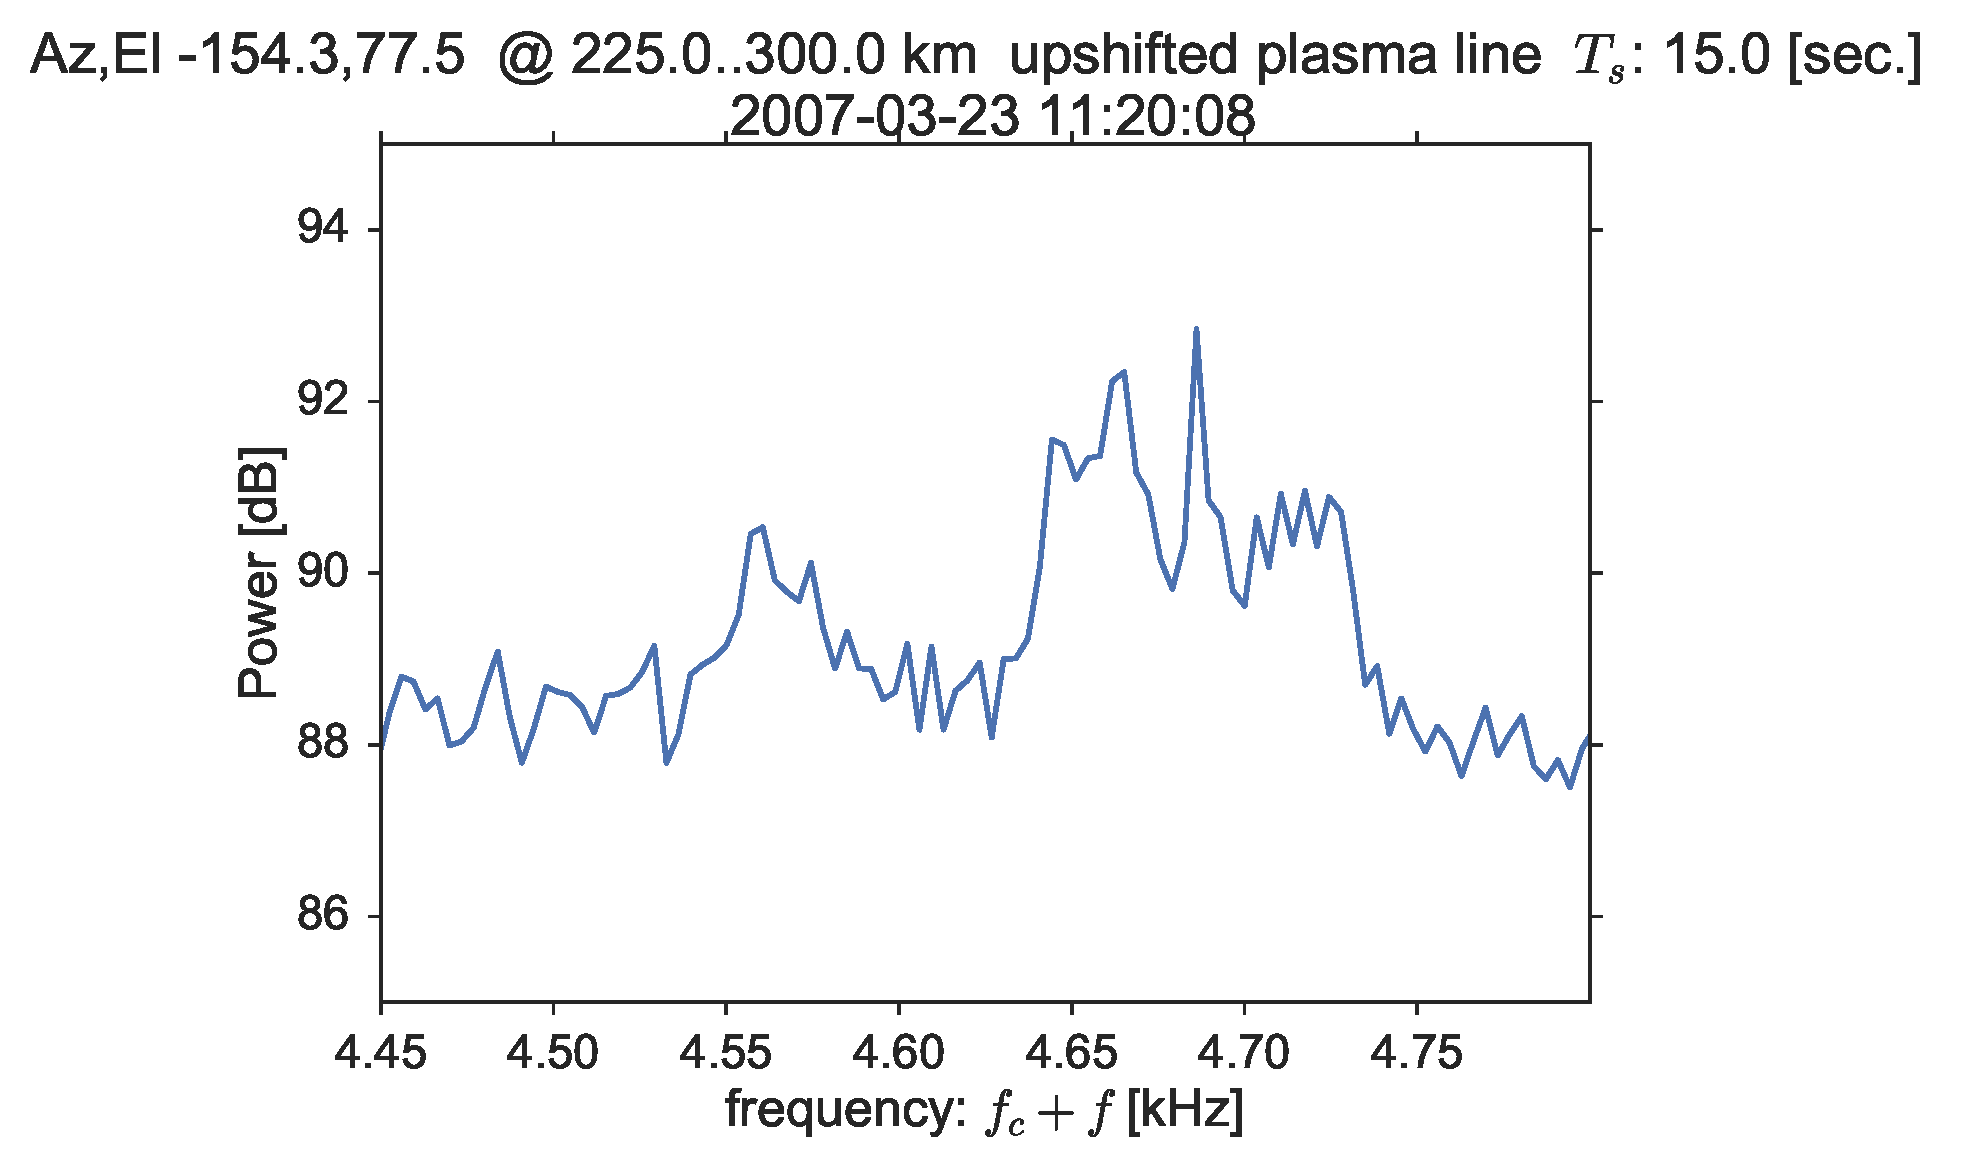
\includegraphics[width=0.45\columnwidth,trim=0 60 0 0]{gfx/2007-03-23/plasmaUPslice2007-03-2311-20-08}
    
    \vspace{-0.5cm}
    \hspace{0.5cm}(i)\hspace{0.425\columnwidth}(j)
    \vspace{0.5cm}
    
    \caption{Substorm breakup: highly dynamic aurora on 23 March 2007. 
        Low-altitude NEIALs observed corresponding to (a,c,f,i,j) with possible Farley-Buneman instability in the E-region. 
        Streaming upflow corresponding to (d,h).
    Strong Langmuir turbulence corresponding to (c,f,g). }\label{fig:20070323}
\end{figure}
The PF-DMSP spectra ratio $I_{6300}/I_{4278}$ in Figure~\ref{fig:mspratio0323} dips as low as 0.02 during the breakup, indicating a large flux with $E_0 > \unit[10]{keV}$ according to \citet{rees1974}.
\begin{sidewaysfigure}\centering
    \includegraphics[width=0.85\linewidth]{gfx/2007-03-23/msp-ratio}
    \caption{PF-DMSP spectral ratio breakup event 2007 March 23 11:22 UTC.
        The ratio $I_{6300}/I_{4278}$ dips as low as 0.02 during the breakup, indicating a large flux with $E_0 > \unit[10]{keV}$ according to \citet{rees1974}.}
    \label{fig:mspratio0323}
\end{sidewaysfigure}
The $I_{5577}/I_{4278}$ in Figure~\ref{fig:mspratio0323-5577} dips as low as 1 during the breakup, also indicating a large flux with $E_0 > \unit[10]{keV}$ according to \citet{rees1974}.
\begin{sidewaysfigure}\centering
    \includegraphics[width=0.85\linewidth]{gfx/2007-03-23/msp-ratio-5577}
    \caption{PF-DMSP spectral ratio breakup event 2007 March 23 11:22 UTC.
        The ratio $I_{5577}/I_{4278}$ dips as low as 1 during the breakup, indicating a large flux with $E_0 > \unit[10]{keV}$ according to \citet{rees1974}.}
    \label{fig:mspratio0323-5577}
\end{sidewaysfigure}
The GIMA magnetometers data surrounding this event is shown in Figure~\ref{fig:20070323mag}, with the expected strong perturbation near the event time.
\begin{figure}
    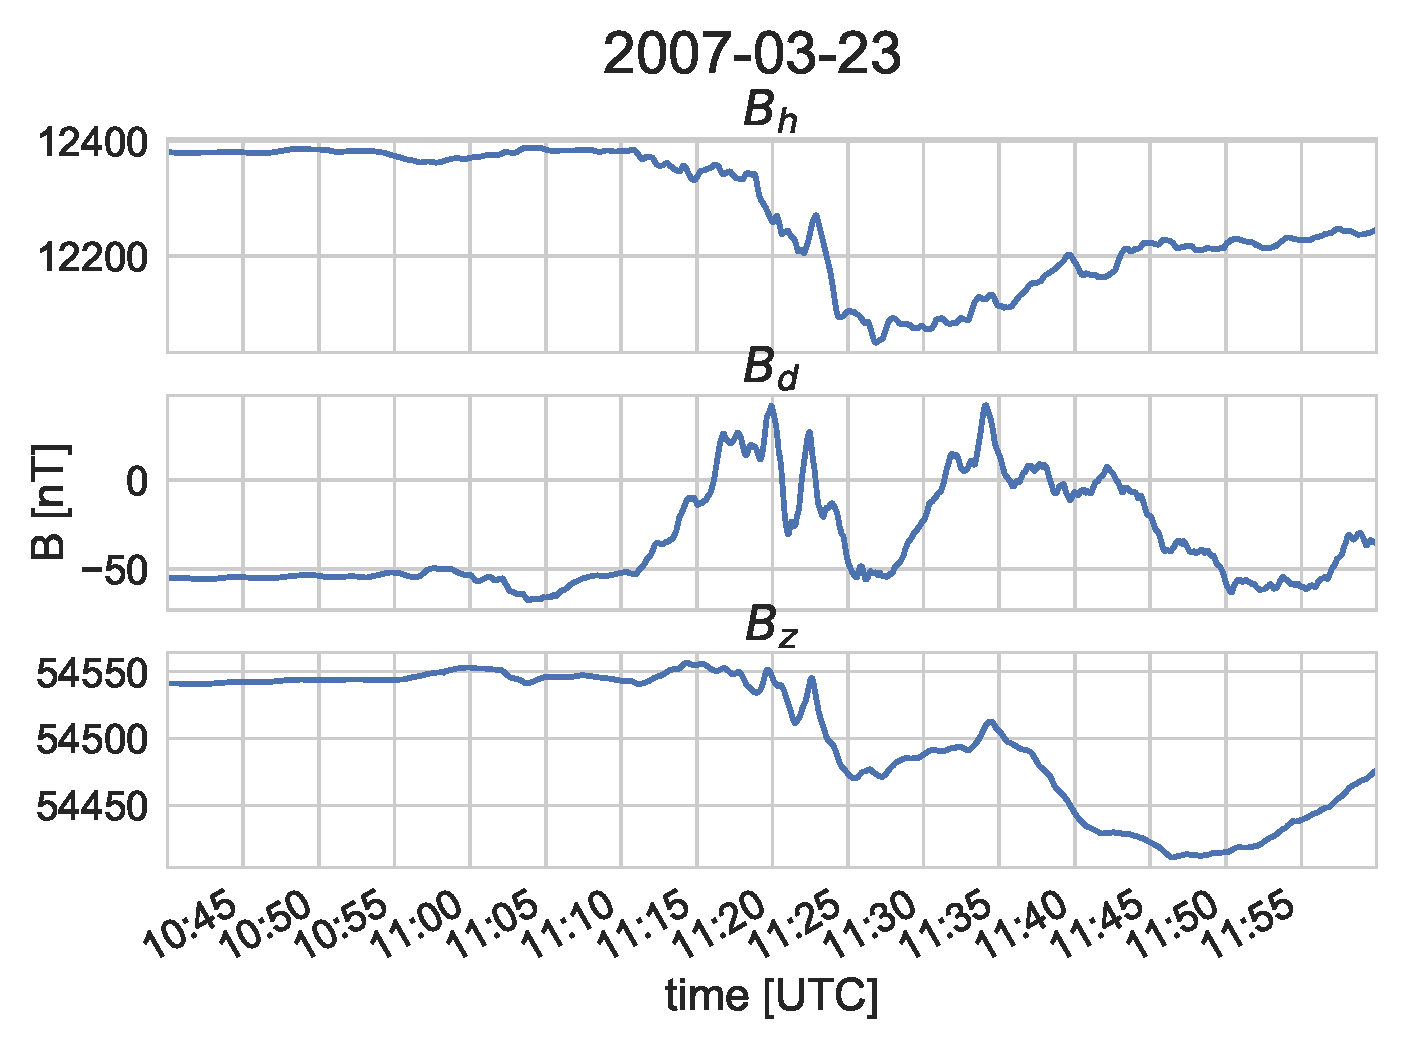
\includegraphics[width=\columnwidth]{gfx/2007-03-23/mag}
    \caption{Strong B-field perturbance due to substorm on 2007-03-23 near 11:20 UTC.}
    \label{fig:20070323mag}
\end{figure}

This was an exceptionally intense breakup event.
This magnificent substorm breakup had splitting arcs embedded in the wildly dynamic behavior captured by PFISR and a single BG3-filtered EMCCD camera. 
This event has been analyzed in detail by \citet{semeter2008,akbari2012}.


\subsection{Splitting Auroral Arcs}\label{sec:split}
One of the ground-observable optical manifestations of a DAW event are bifurcating ``shedding'' or ``splitting'' arcs, which have a pattern of one or more spatiotemporal leaves folding off of the main arc. 
During the shedding event of Figures~\ref{fig:20130414T0854a}-\ref{fig:20130414T0854b}, PFISR power in the magnetic zenith beam (represented by a red circle in Figure~\ref{fig:20130414T0854a}(a-d)) is enhanced by over \unit[25]{dB} in the F-region ionosphere above the bifurcation zone.
\begin{sidewaysfigure}\noindent

    \includegraphics[width=\columnwidth,trim=0 680 0 50,clip]{gfx/2013-04-14T0854/2013-04-14T0854}\\
    
    \vspace{-1.175cm}
    \hspace{1.35cm}{\color{white}(a) 08:54:16}
    \hspace{2.1cm}{\color{white}(b) 08:54:21}
    \hspace{2.15cm}{\color{white}(c) 08:54:26}
    \hspace{2.15cm}{\color{white}(d) 08:54:31}
    \vspace{0.5cm}
    
    % backscatter
    \begin{center}
    \includegraphics[width=0.9\columnwidth,trim=10 0 0 185,clip]{gfx/2013-04-14T0854/power_longpulse2013-04-1408-54}\\
    \end{center}
    
    \vspace{-1.5cm}
    (e) 
    \vspace{.5cm}
      
    \caption{Splitting auroral arc sequence at PFISR, April 14, 2013. 
        (a) beginning of plasma turbulence bursts.
        (b) F-region ionization increasing nearly \unit[30]{dB} above background. 
        The turbulence fades in (c), enhancing to even greater intensity in (d) for ten seconds.
        (e) backscattered ISR power.}
    \label{fig:20130414T0854a}
\end{sidewaysfigure} 

\begin{figure}\noindent
	   % psd ion-line 
	\includegraphics[width=0.425\columnwidth]{gfx/2013-04-14T0854/acfslice_longpulse2013-04-1408-54-16}
	\includegraphics[width=0.425\columnwidth]{gfx/2013-04-14T0854/acfslice_longpulse2013-04-1408-54-31}\\
	
	\vspace{-1.5cm}
	\hspace{0.0cm}(a)\hspace{0.4\columnwidth}(b)
	\vspace{0.3cm}
	
	% down-shift
	\includegraphics[width=0.425\columnwidth,trim=0 50 0 0]{gfx/2013-04-14T0854/plasmaDOWNslice2013-04-1408-54-16}
	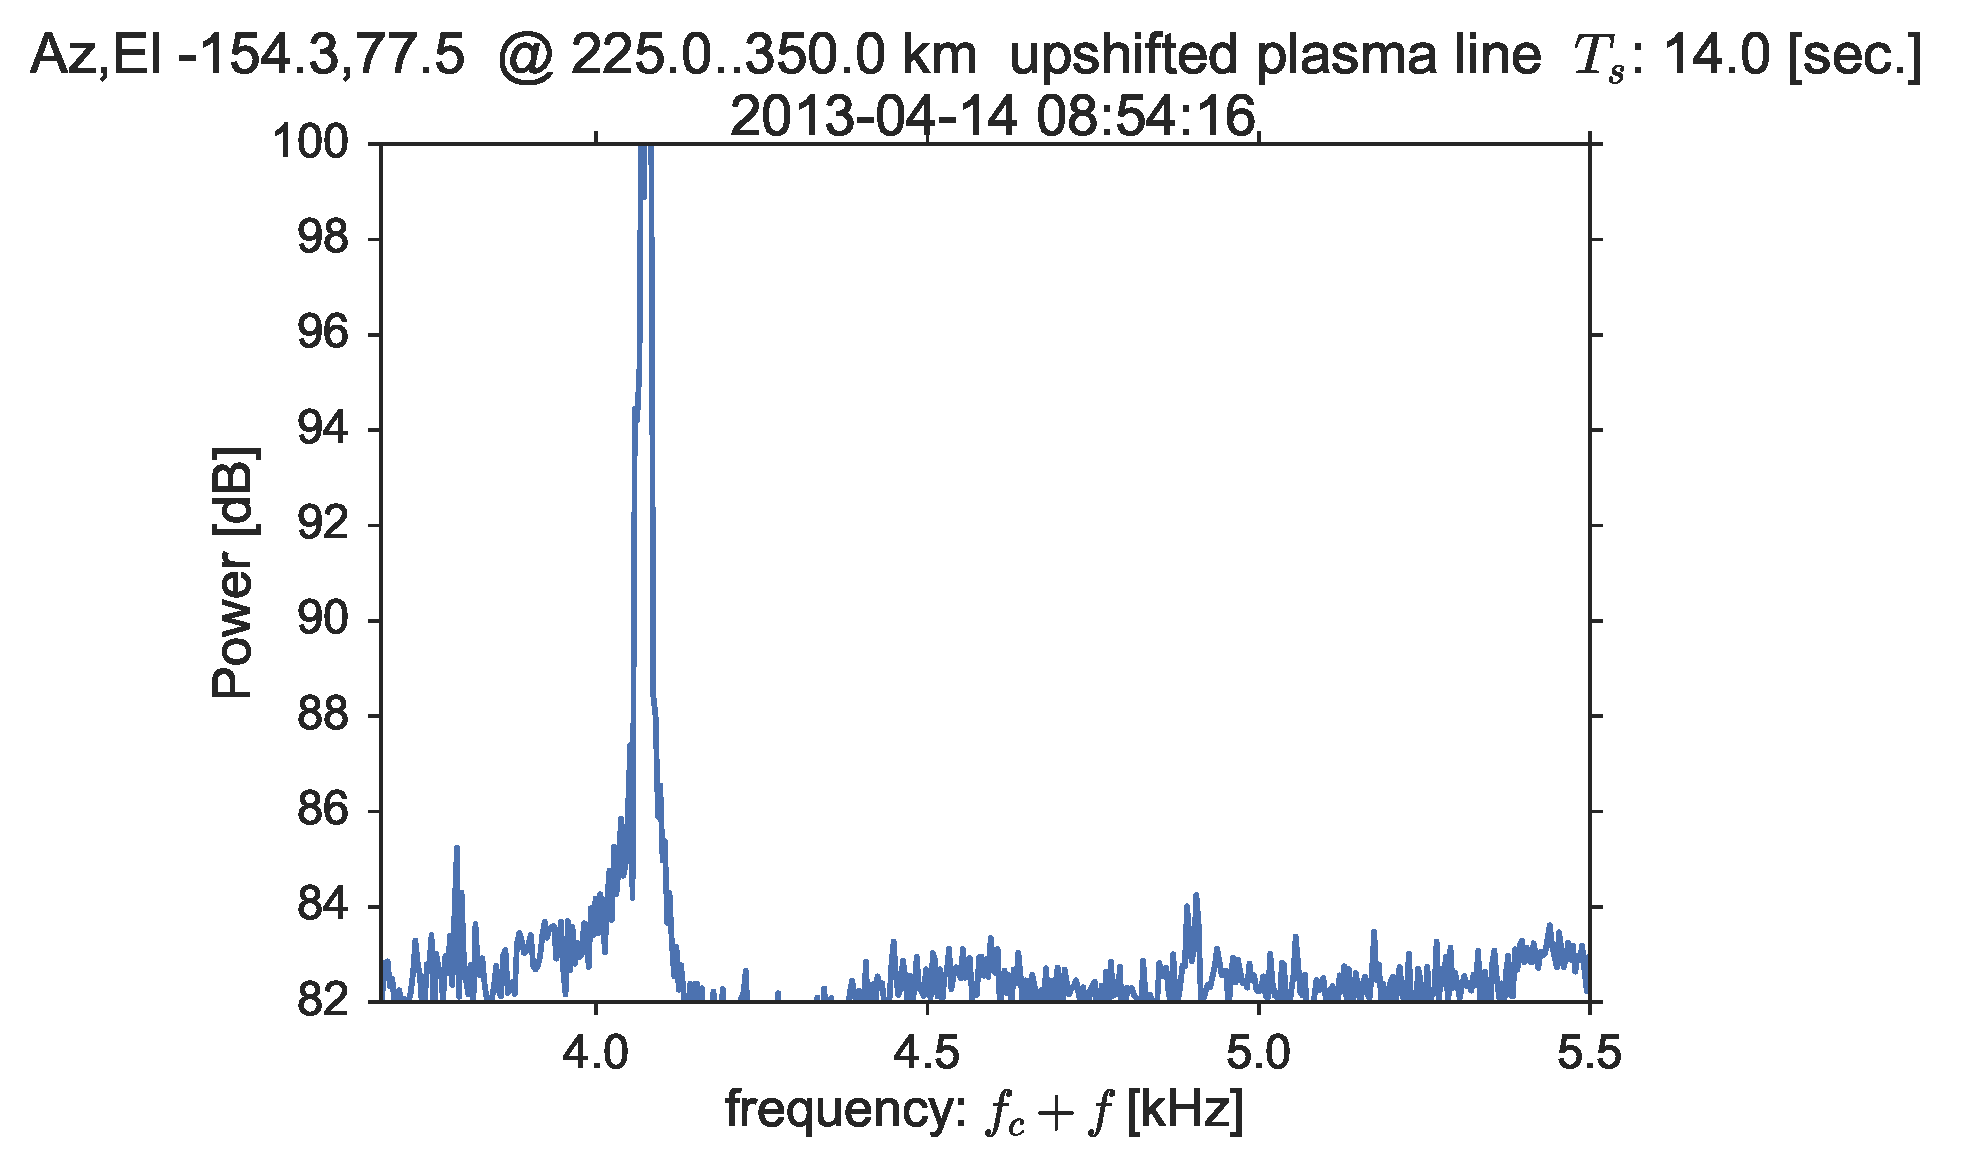
\includegraphics[width=0.425\columnwidth,trim=0 50 0 0]{gfx/2013-04-14T0854/plasmaUPslice2013-04-1408-54-16}\\
	
	\vspace{-1.2cm}
	\hspace{0.0cm}(c)\hspace{0.4\columnwidth}(d)
	\vspace{0.3cm}
	
	% up-shift
	\includegraphics[width=0.425\columnwidth,trim=0 50 0 0]{gfx/2013-04-14T0854/plasmaDOWNslice2013-04-1408-54-31}
	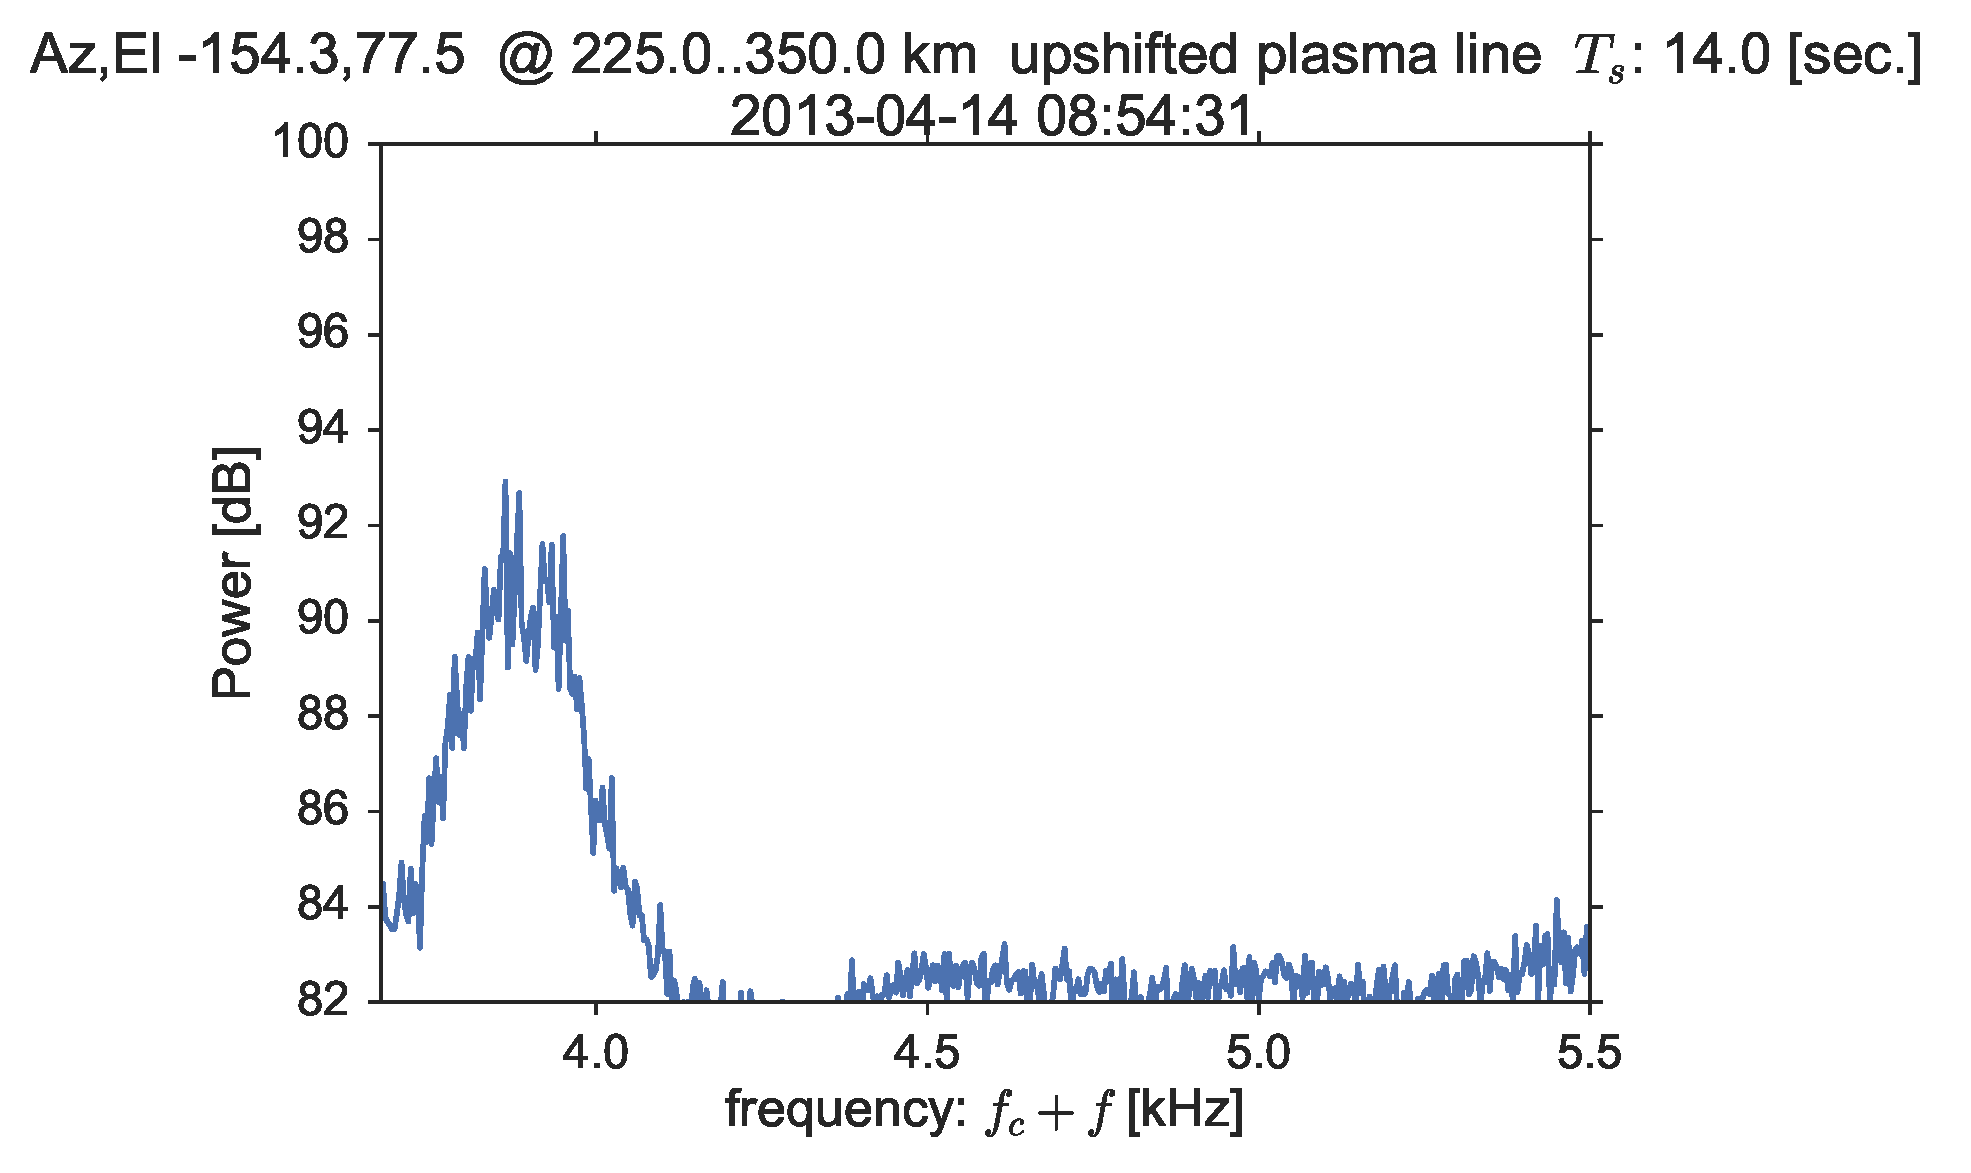
\includegraphics[width=0.425\columnwidth,trim=0 50 0 0]{gfx/2013-04-14T0854/plasmaUPslice2013-04-1408-54-31}\\
	
	\vspace{-1.2cm}
	\hspace{0.0cm}(e)\hspace{0.4\columnwidth}(f)
	\vspace{0.3cm}
	
	\caption{Splitting auroral arc sequence at PFISR, April 14, 2013.
		(a,b) backscattered power related to (a-c) and (d) respectively.
		(c,d) down- and up-shifted plasma line enhancements corresponding to Figure~\ref{fig:20130414T0854a}(a-c).
		(e,f) down- and up-shifted plasma line enhancements corresponding to Figure~\ref{fig:20130414T0854a}(d).}
	\label{fig:20130414T0854b}
\end{figure}
On the night of April 14, 2013, several instruments with diverse observing modalities were active in the vicinity of PFRR, as depicted in Figure~\ref{fig:sitemap}. 
PFISR and DASC are co-located, so the center of the PFISR beams in the image can be taken as approximately constant.
The GIMA magnetometer data is shown in Figure~\ref{fig:gima0854}, showing the usual southward IMF in the time vicinity of the splitting arc.
\begin{figure}
	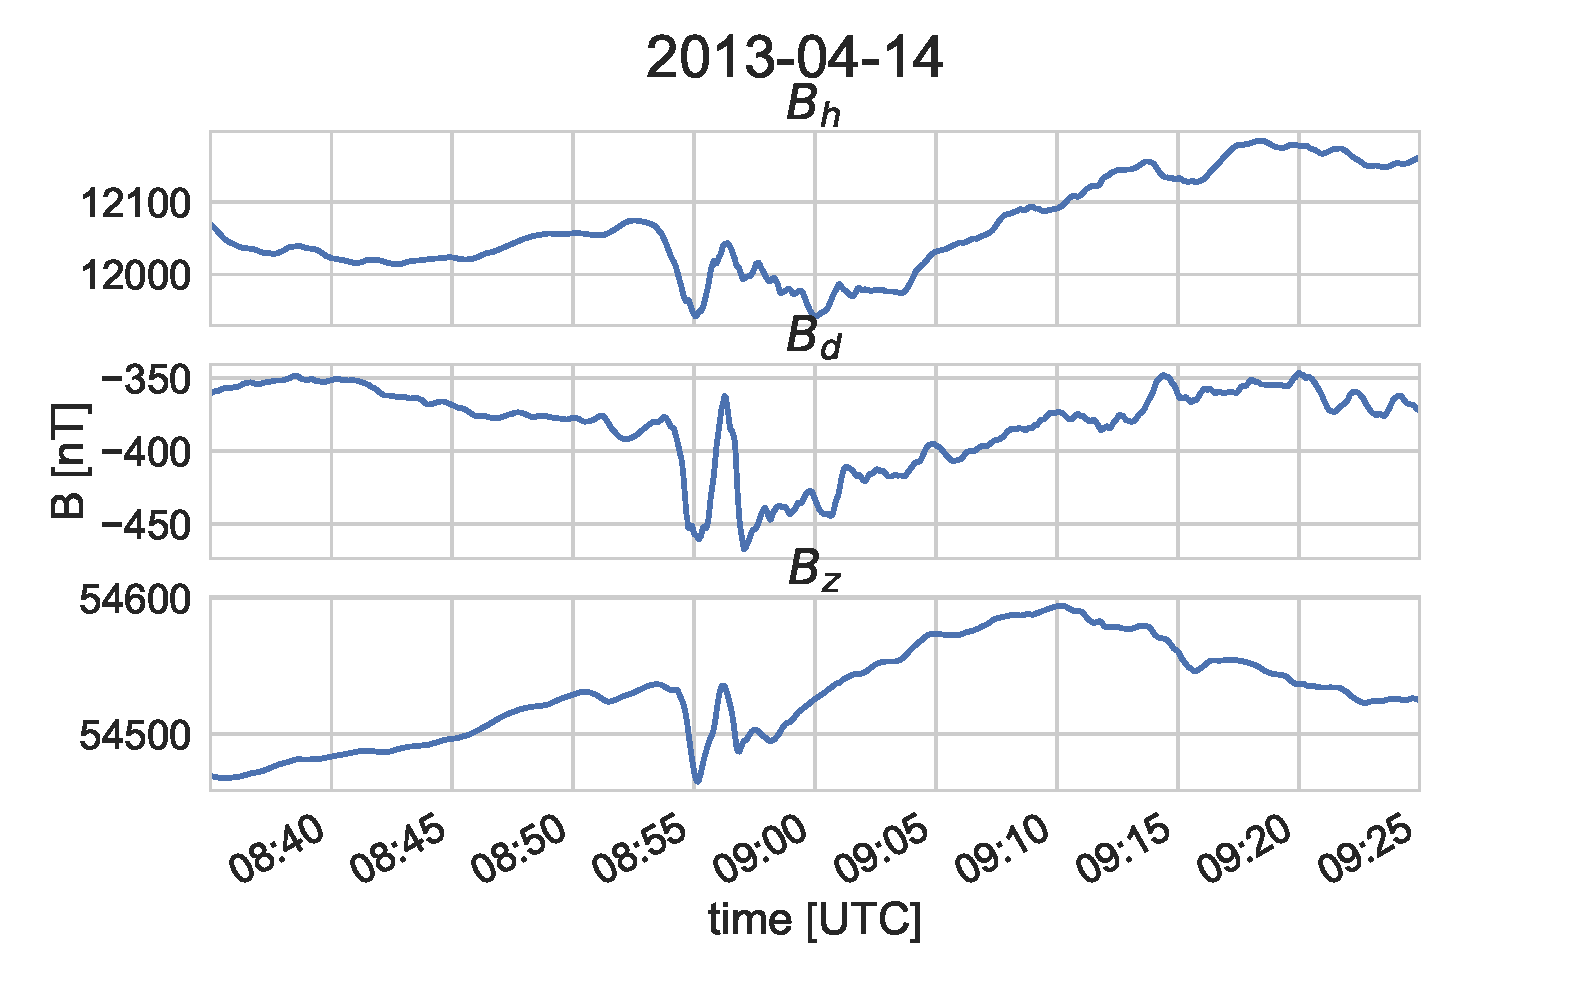
\includegraphics[width=\columnwidth]{gfx/2013-04-14T0854/mag}
	\caption{PFRR GIMA magnetometer data for 2013-04-14 showing evidence of southward IMF in time vicinity of splitting arc.}
	\label{fig:gima0854}
\end{figure}


Observe in Figure~\ref{fig:20130414T0854b}(c-f) that only the plasma line spectra for 08:54:16 and 08:54:31 UT show prominent reflections from plasma turbulence.
The rest of the plasma line spectra near this time looks much like the 08:54:45 data.
%In contrast, the ion line spectrum in Figure~\ref{fig:20130414T0854}(f,g,h) still shows the turbulence effects at 08:54:45, so an earlier frame at 08:54:02 UT is included to show the non-turbulent ion line spectra.
%A movie sequence for this event is available in the Supplemental Materials for this article.
We integrate the received ISR power over the NEIALs altitude range and plot this integrated measurement with the HiST optical data. 
It is initially apparent from comparing Figure~\ref{fig:20130414T0854a}(a-d) with Figure~\ref{fig:20130414T0854a}(e) that the highest SNR bursts come from the times when the magnetic zenith ISR beam is over a region of optically ``shedding'' arcs.
Figure~\ref{fig:20130414T0854a}(a) depicts a typical dispersive Alfvén wave auroral scene. 
The red circle denotes local magnetic zenith. 
Observe the fine spatial structure along the $B_\perp$ direction. 
Figure~\ref{fig:shedintion}(b) shows the plasma line summed over altitudes from \unit[200..350]{km}.
Figure~\ref{fig:20130414T0854b}(a,b) shows the ion line PSD during the time of this shedding auroral event--observe the ``flat top'' characteristic of the spectrum seen only during NEIALs.

Turning to optical spectral information, the PF-DMSP data in Figure~\ref{fig:shedratio0854}(a-b) is used to compare \unit[427.8]{nm} intensity from N$_2^+$ $I_{427.8}$ with prompt OI emissions at \unit[630.0]{nm} $I_{630.0}$.
This ratio in Figure~\ref{fig:shedratio0854}(c) shows that just before and during the splitting arc, $I_{427.8}$ is nearly twice as strong as $I_{630.0}$. 
\begin{figure}
    \includegraphics[width=\columnwidth,trim=3 3 3 3,clip]{gfx/2013-04-14T0854/MSPintensityratio}
    \caption{PF-DMSP (a) $I_{630.0}$ and (b) $I_{427.8}$ emission intensity with (c) $I_{630.0}/I_{427.8}$ emission intensity ratio at 08:54 UT during the 14 April 2013 substorm. Golden dashed lines refer to approximate elevation FOV of HiST cameras.}\label{fig:shedratio0854}
\end{figure}
After the splitting event completes, the \unit[630.0]{nm} line once again dominates $I_{427.8}$ by a factor of 1.5 to 3.5 as was also the case before the splitting began.
Figure~\ref{fig:shedratioplot0854} provides an alternative view of $I_{630.0}$/$I_{427.8}$.
\begin{figure}
    \includegraphics[width=0.9\columnwidth]{gfx/2013-04-14T0854/msp_ratio}
    \caption{PF-DMSP ratio of $I_{630.0}/I_{427.8}$ emission intensity ratio with one line plot per time. Observe that high energy beam (indicated by lowest ratio at 08:54:10) does not immediately lead to splitting arc. It takes about 10 seconds for visible arc splitting to occur. Golden dashed lines refer to approximate elevation FOV of HiST cameras.}
    \label{fig:shedratioplot0854}
\end{figure}
%These measurements are within the typical range for $I_{630.0}$ and $I_{427.8}$~\citep{Dashkevich2006}.
From \citet{rees1974}, at 08:54:10 UTC at the magnetic zenith angle of $102.5^\circ$ elevation from north, $I_{630.0}/I_{427.8} \sim 0.6$, corresponding to a characteristic energy of \unit[1.6]{keV} for the assumptions on neutral composition and brightness observed.

Historical work has often relied on spectrometer readings for estimates of characteristic energy $E_0$, represented in Figure~\ref{fig:alfvenflux} as the high-energy ``bump''.
Historically these measurements had cadences of several seconds, and obviously lacked a sense of the auroral morphology.
As the extensive literature referenced throughout this paper has noted, quantitative correlation of auroral spatio-temporal evolution with plasma turbulence requires an FOV of several degrees about magnetic zenith with at least 40 frames/s sampling, and with filtering sufficient to remove the blur of metastable emissions \citep{hirsch2016}.
The tomography data inversion exemplified in Figures~\ref{fig:histfwd} and \ref{fig:histest} is an example of the new capabilities afforded by HiST for such applications.
\begin{sidewaysfigure}\centering
    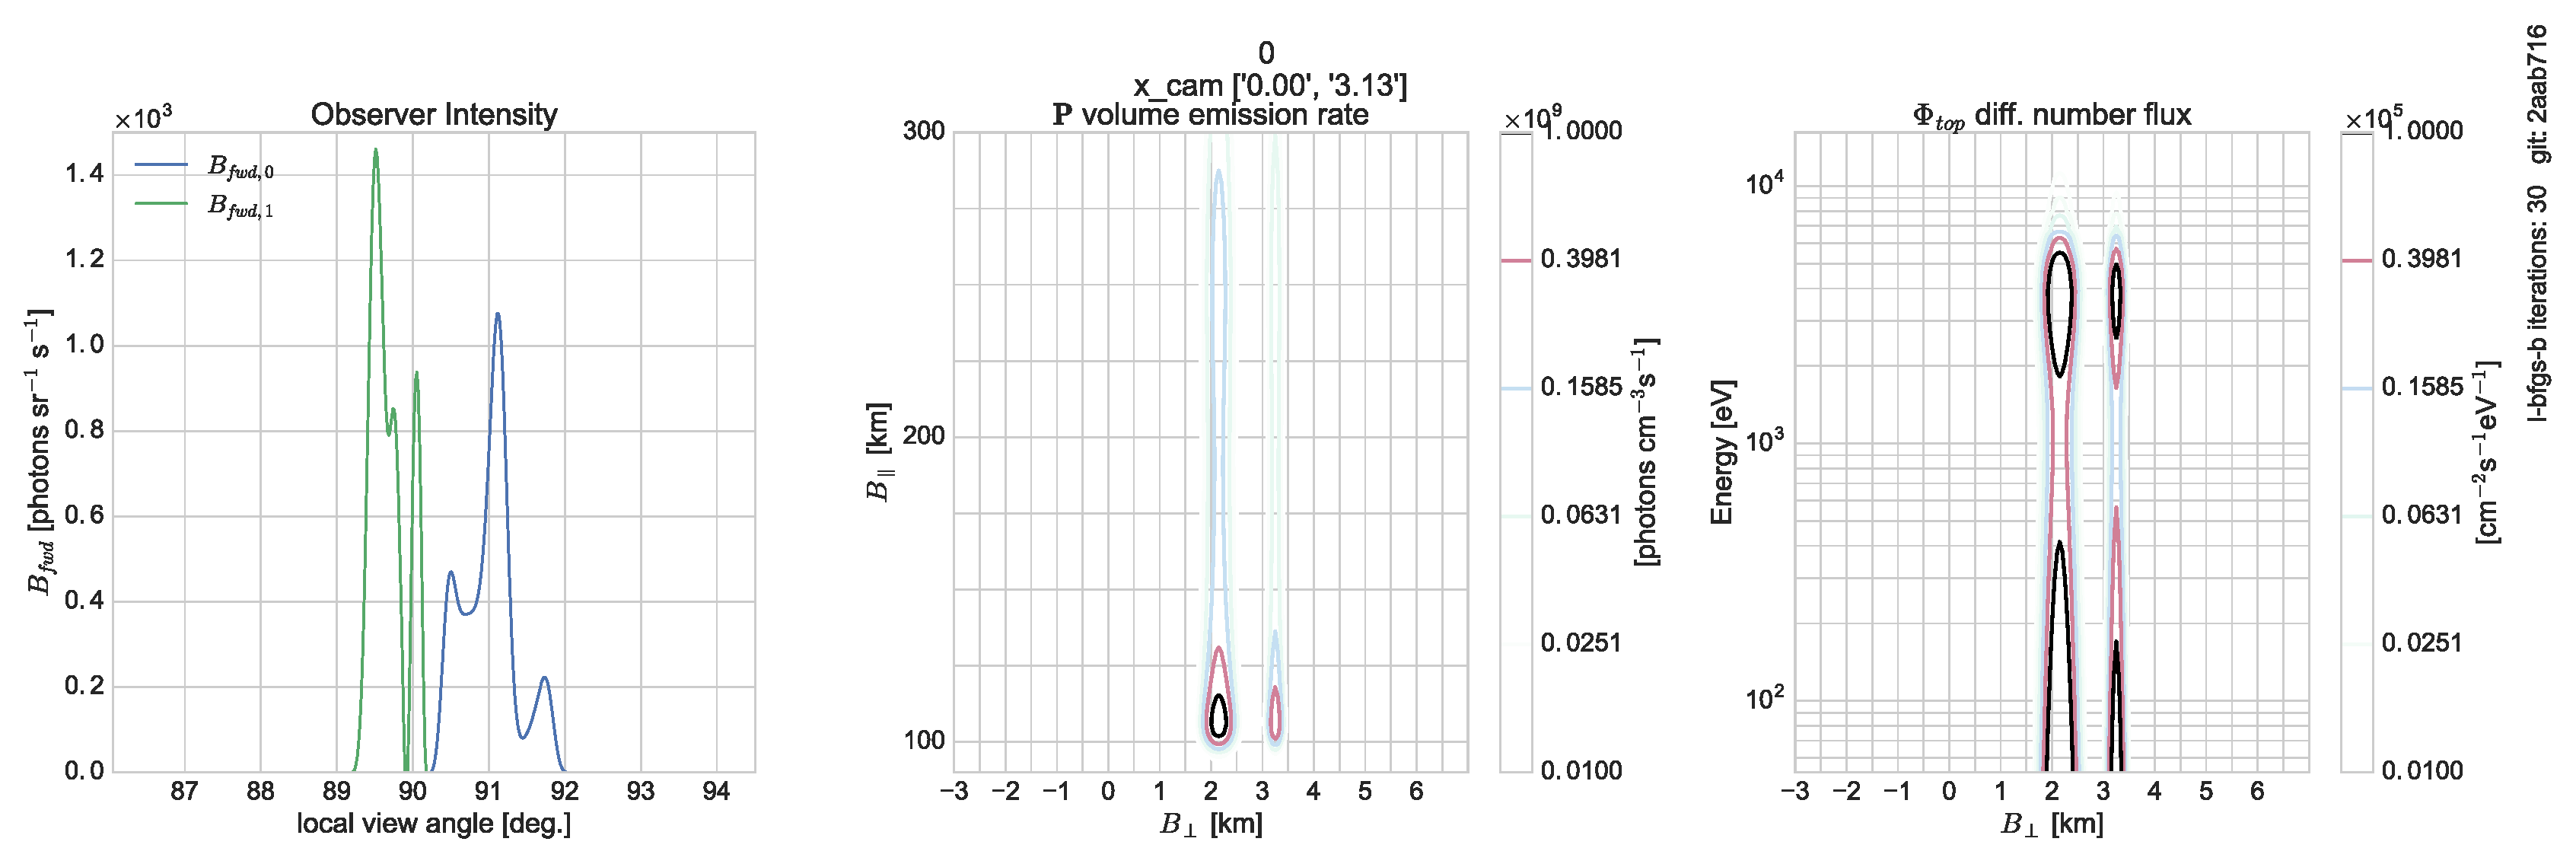
\includegraphics[width=0.9\columnwidth]{gfx/fwd0}
    \caption{Forward model of aurora for HiST two-camera deployment at PFRR. Splitting arc is simulated. 
    	Panel (a) shows ground-observed optical intensity after filtering and wavelength-dependent atmospheric attenuation. 
    	(b) shows the auroral optical volume emission rate vs. $B_\perp$. 
    	(c) shows the unobservable primary electron differential number flux at the ``top'' of the ionosphere, this is the quantity the HiST system estimates with high spatiotemporal resolution.}\label{fig:histfwd}
\end{sidewaysfigure}
\begin{sidewaysfigure}\centering
    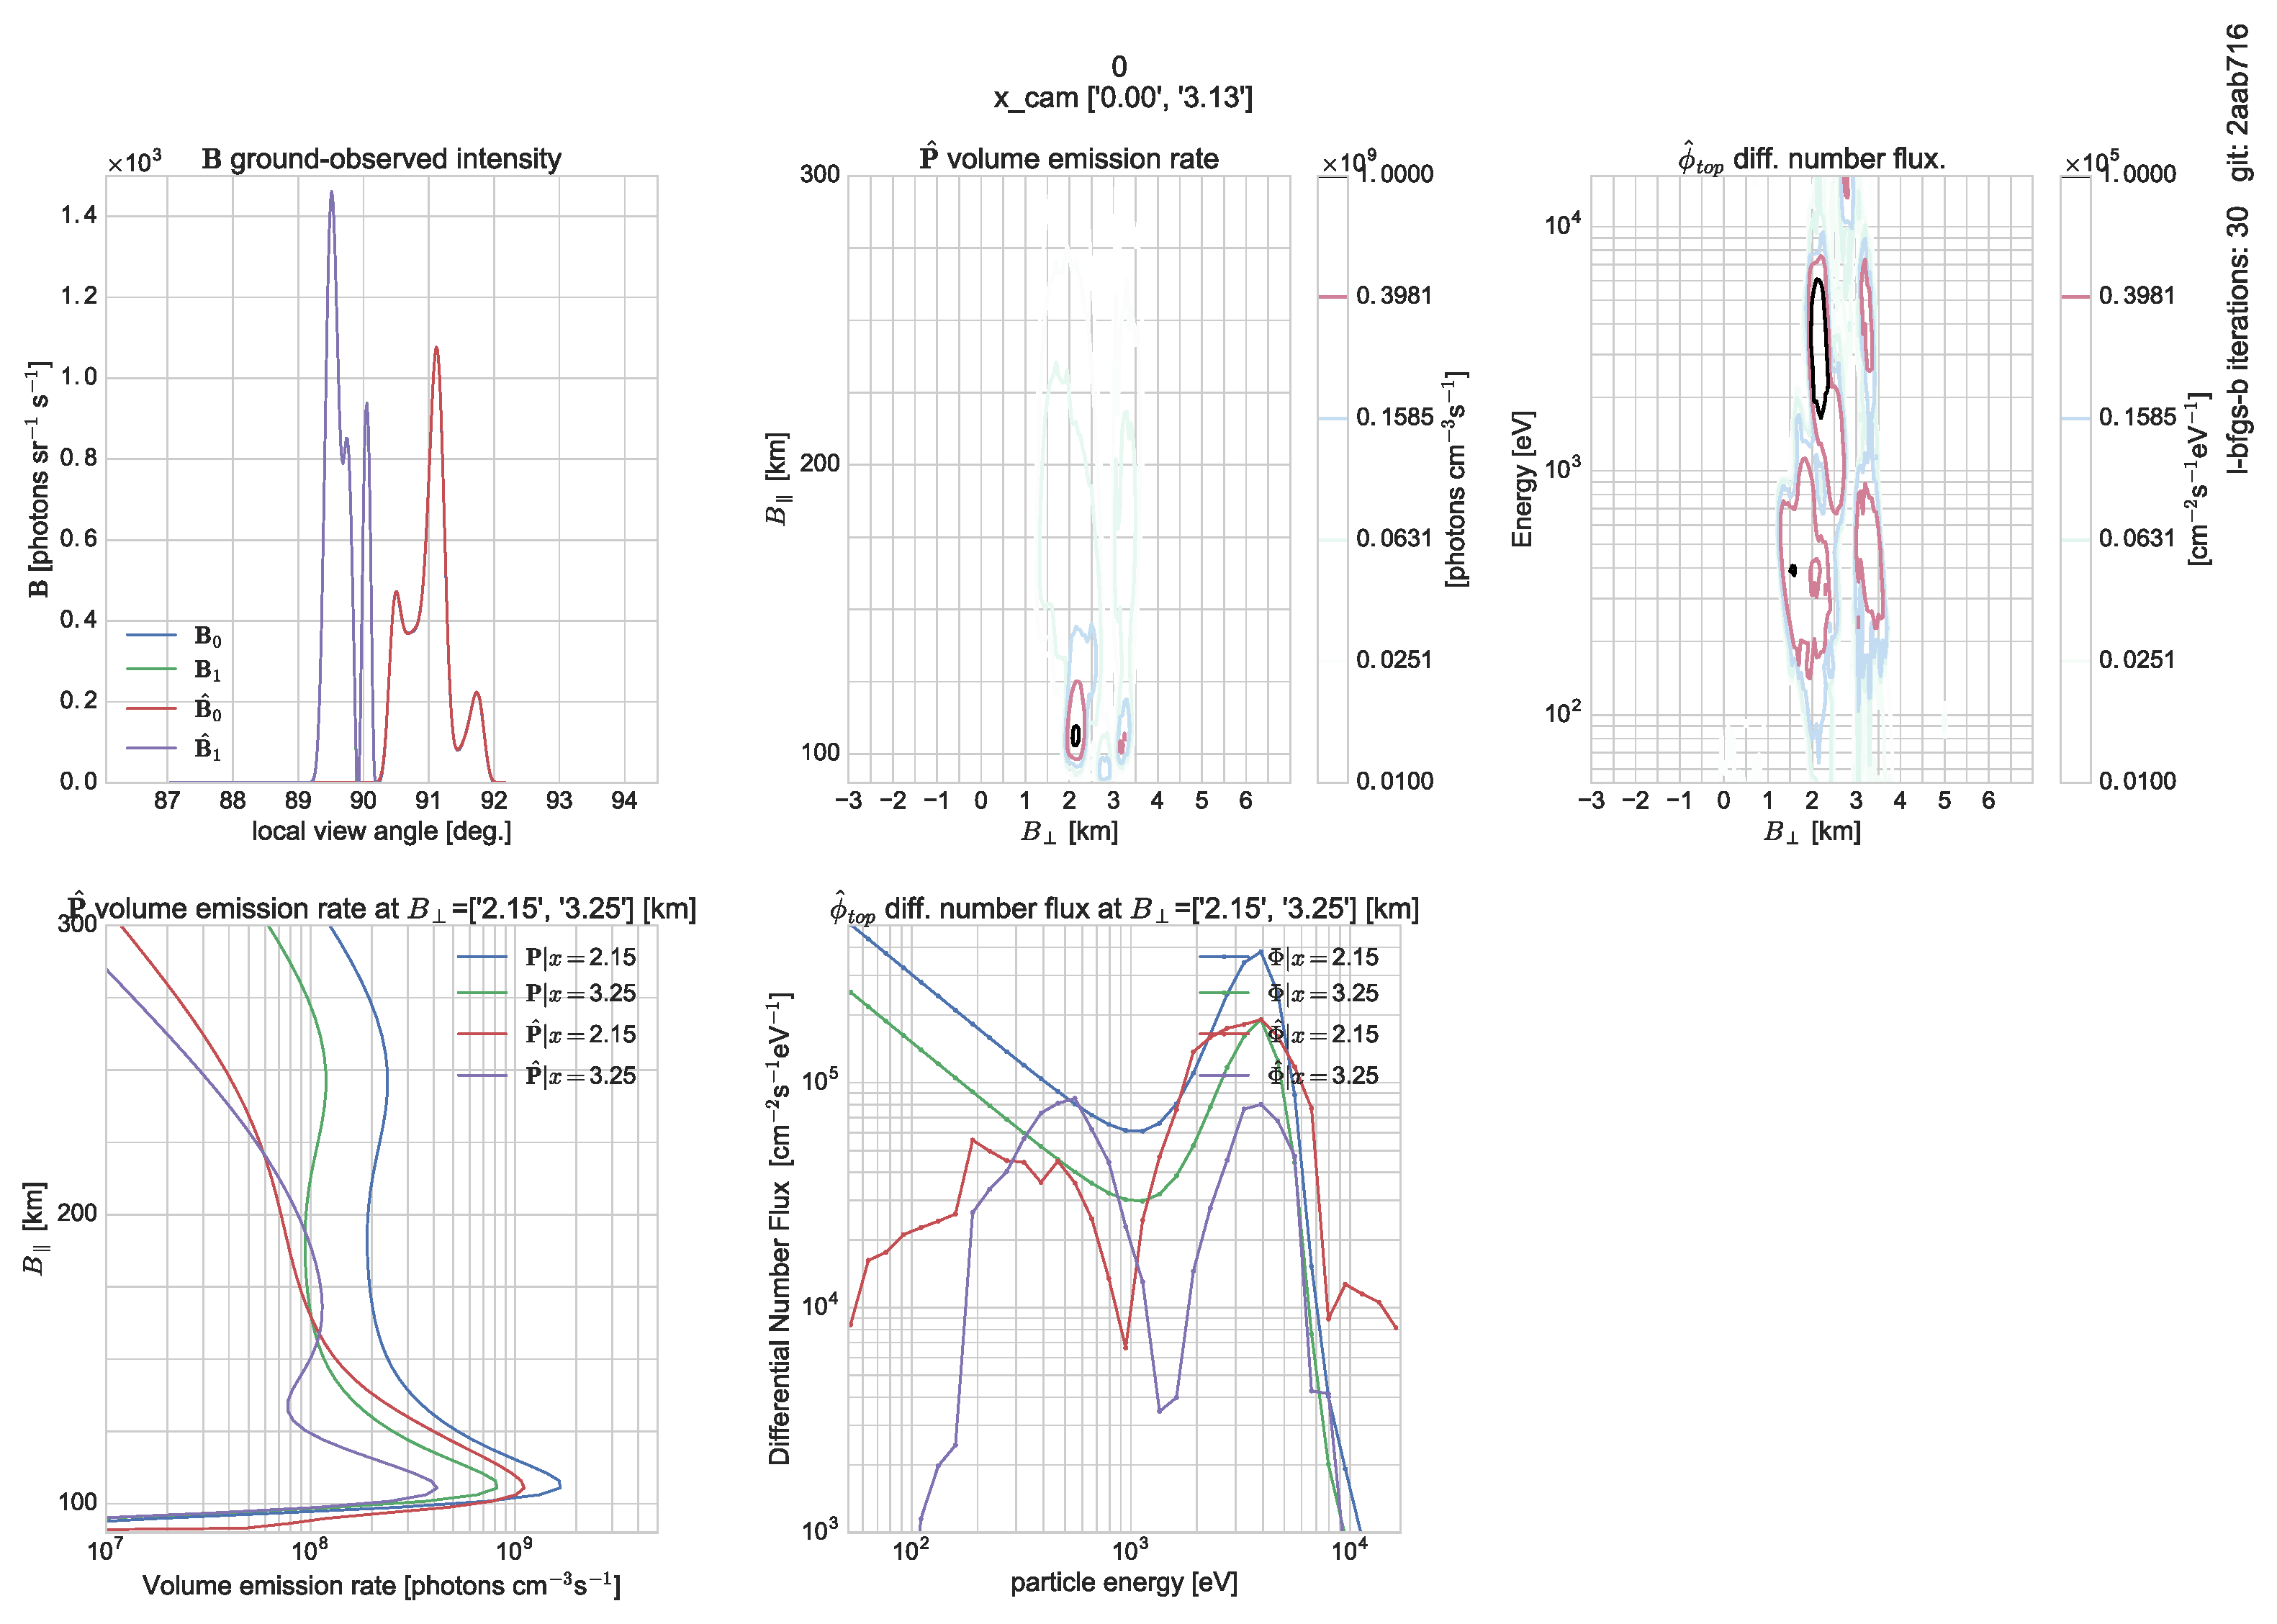
\includegraphics[width=0.75\columnwidth]{gfx/est0}
    \caption{Data inversion for forward modeled HiST two-camera deployment at PFRR. Splitting arc is simulated as in Figure~\ref{fig:histfwd} and precipitation estimated. Panel (a) shows ground-observed and estimated optical intensity after filtering and wavelength-dependent atmospheric attenuation. (b) shows the estimated auroral optical volume emission rate vs. $B_\perp$. (c) shows the estimated primary electron differential number flux at the ``top'' of the ionosphere. (d) shows a 1-D vertical cut of volume emission rate for the two arcs, forward model and estimated. (e) shows a 1-D cut in $B_\perp$ for each arc, forward model and estimated differential number flux.}\label{fig:histest}
\end{sidewaysfigure}

\subsection{Flaming auroral arcs}\label{sec:fusflame}
Flaming aurora manifests as rapidly increasing peak brightness altitude.
The effect can have an appearance like the rapidly rising flames of a campfire, leading to the name for this auroral morphology.
The driving factor behind flaming aurora is dispersive Alfvén waves.
The high energy precipitating particles arrive first in the auroral altitudes of the ionosphere, followed $\sim \unit[100]{ms}$ later by the lower energy particles.

An example flaming auroral arc occurred at PFISR on March 1, 2011 near 10:06 UTC.
Figure~\ref{fig:20110301a}(a) shows pre-Alfvénic arc configuration.
F-region irregularities starting below \unit[300]{km} and rising up to \unit[600]{km} within two seconds are observed in Figure~\ref{fig:20110301a}(b) ISR power with the arrival of high-energy dispersive Alfvénic particles.
\unit[400]{ms} later in Figure~\ref{fig:20110301a}(c), the low-energy Alfvénic flux dominates as the apparent peak altitude of prompt emissions rises rapidly.
Figure~\ref{fig:20110301b}(a) shows the ion-line during the NEIAL altitude climb, with (g) after the NEIAL rose to a more steady altitude.
A few seconds later in Figure~\ref{fig:20110301a}(d), the Alfvénic particle packet has vanished.
Figure~\ref{fig:20110301b}(c) shows the ion-line spectrum without NEIALs present.
Observe that two more NEIAL events occurred before and after the video, but due to the human-initiated record cycle, they were not recorded with video.
\begin{sidewaysfigure}\centering
    % Video
    \includegraphics[width=0.19\columnwidth,trim=30 0 200 0,clip]{gfx/2011-03-01/2040}
    \includegraphics[width=0.261\columnwidth,trim=30 0 60 0,clip]{gfx/2011-03-01/6440}
    \includegraphics[width=0.261\columnwidth,trim=30 0 60 0,clip]{gfx/2011-03-01/6840}
    \includegraphics[width=0.261\columnwidth,trim=30 0 60 0,clip]{gfx/2011-03-01/10440}
    % Power
    \includegraphics[width=\columnwidth,trim=0 50 0 0]{gfx/2011-03-01/power_longpulse2011-03-0110-06-00}\\
    {\large(e)}
    \vspace{0.1cm}

    \caption{Flaming auroral arc sequence at PFISR on March 1, 2011, 10:06 UTC.
        (a) shows pre-Alfvénic arc configuration.
        (b) F-region irregularities are observed in the ISR power (e) with the arrival of high-energy DAW accelerated electron.
        (c) \unit[400]{ms} later, the low-energy Alfvénic flux dominates as the apparent peak altitude of prompt emissions rises rapidly.
        (d) the Alfvénic particle packet has vanished.
        (e) ISR backscatter showing three NEIAL events in series--video only available for middle event.}
    \label{fig:20110301a}
\end{sidewaysfigure}

\begin{figure}\centering
    % Psd
    \includegraphics[width=0.5\columnwidth,trim=0 50 0 0]{gfx/2011-03-01/acfslice_longpulse2011-03-0110-06-11}

    \vspace{-1cm}(a)
    \vspace{1cm}

    \includegraphics[width=0.5\columnwidth,trim=0 50 0 0]{gfx/2011-03-01/acfslice_longpulse2011-03-0110-06-17}

    \vspace{-1cm}(b)
    \vspace{1cm}

    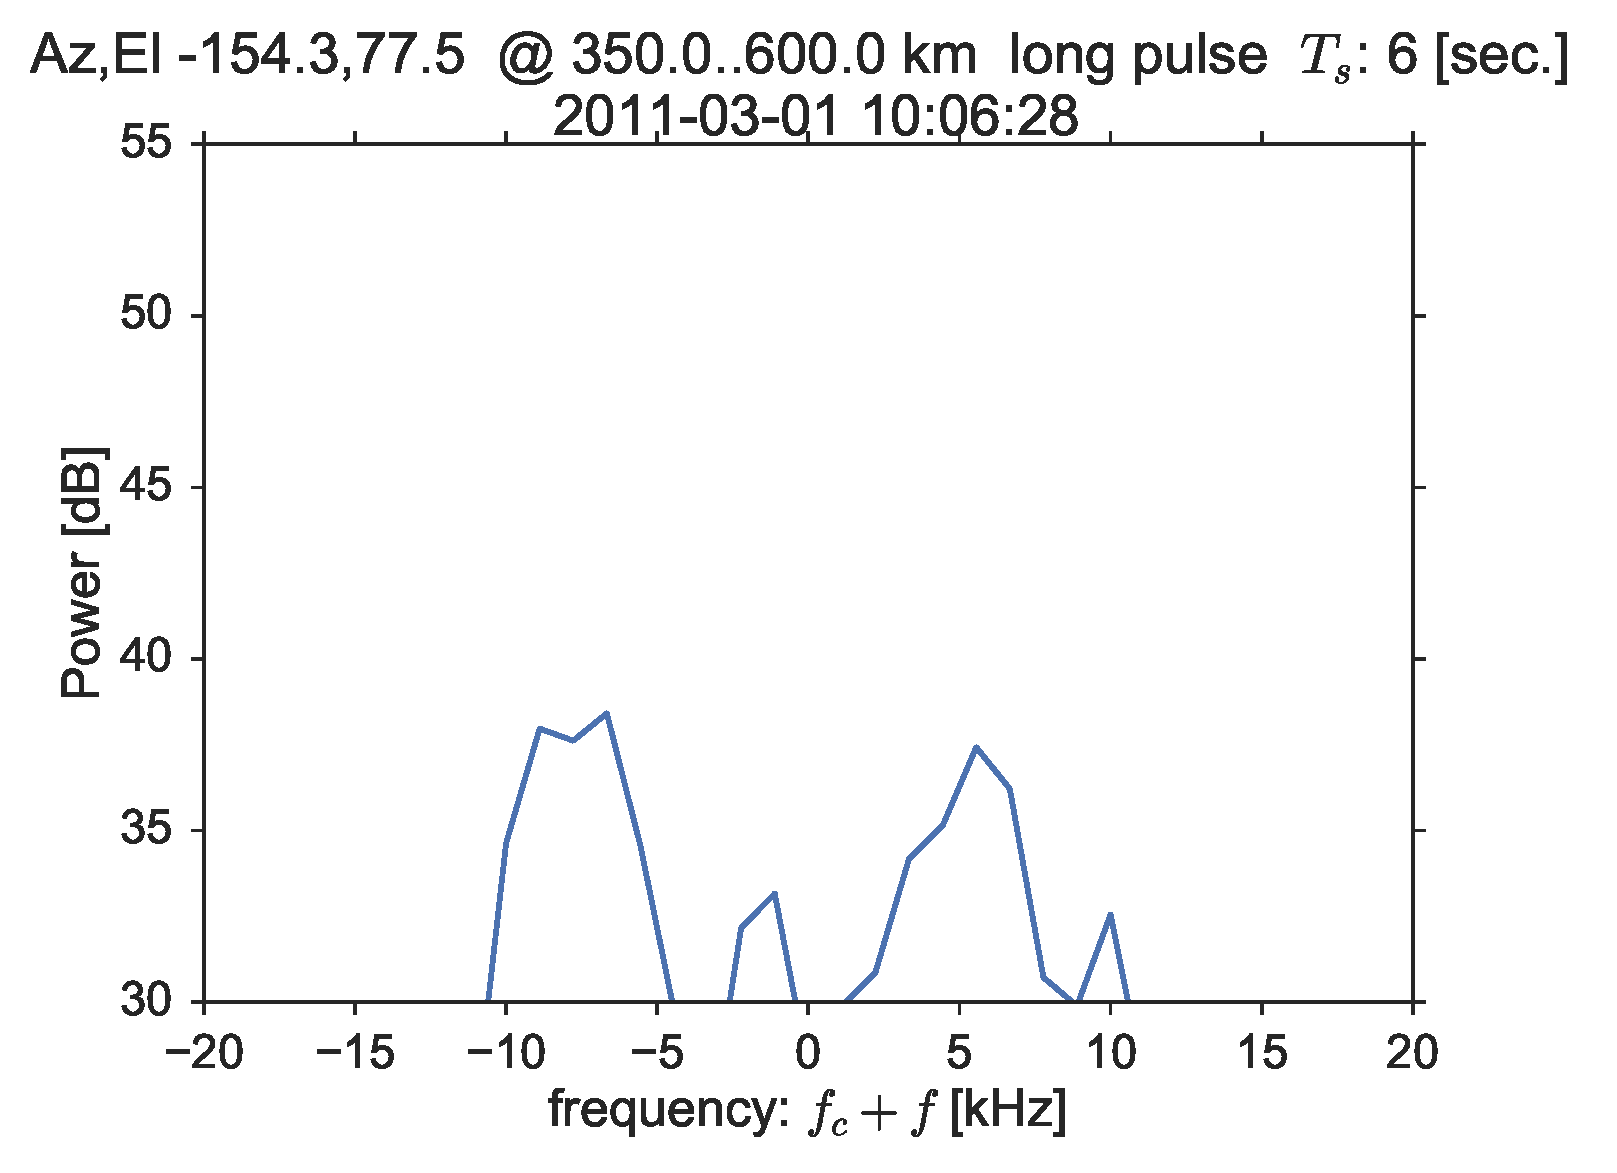
\includegraphics[width=0.5\columnwidth,trim=0 50 0 0]{gfx/2011-03-01/acfslice_longpulse2011-03-0110-06-28}

    \vspace{-1cm}(c)
    \vspace{1cm}

	%(a)\hspace{0.275\columnwidth}(b)\hspace{0.275\columnwidth}(c)

	\caption{Flaming auroral arc sequence at PFISR on March 1, 2011.
    (a,b) show enhanced negative frequency shift ion-acoustic line.
    (c) shows normal ion-acoustic line.}
    \label{fig:20110301b}
\end{figure}

Only a single high-speed sCMOS was running at 30 frames/s, in burst recording mode of several seconds each manual record start.
Context for the event is provided by PF-DMSP in Figure~\ref{fig:msp20110301} and GIMA in Figure~\ref{fig:mag20110301}.
\begin{figure}\centering
    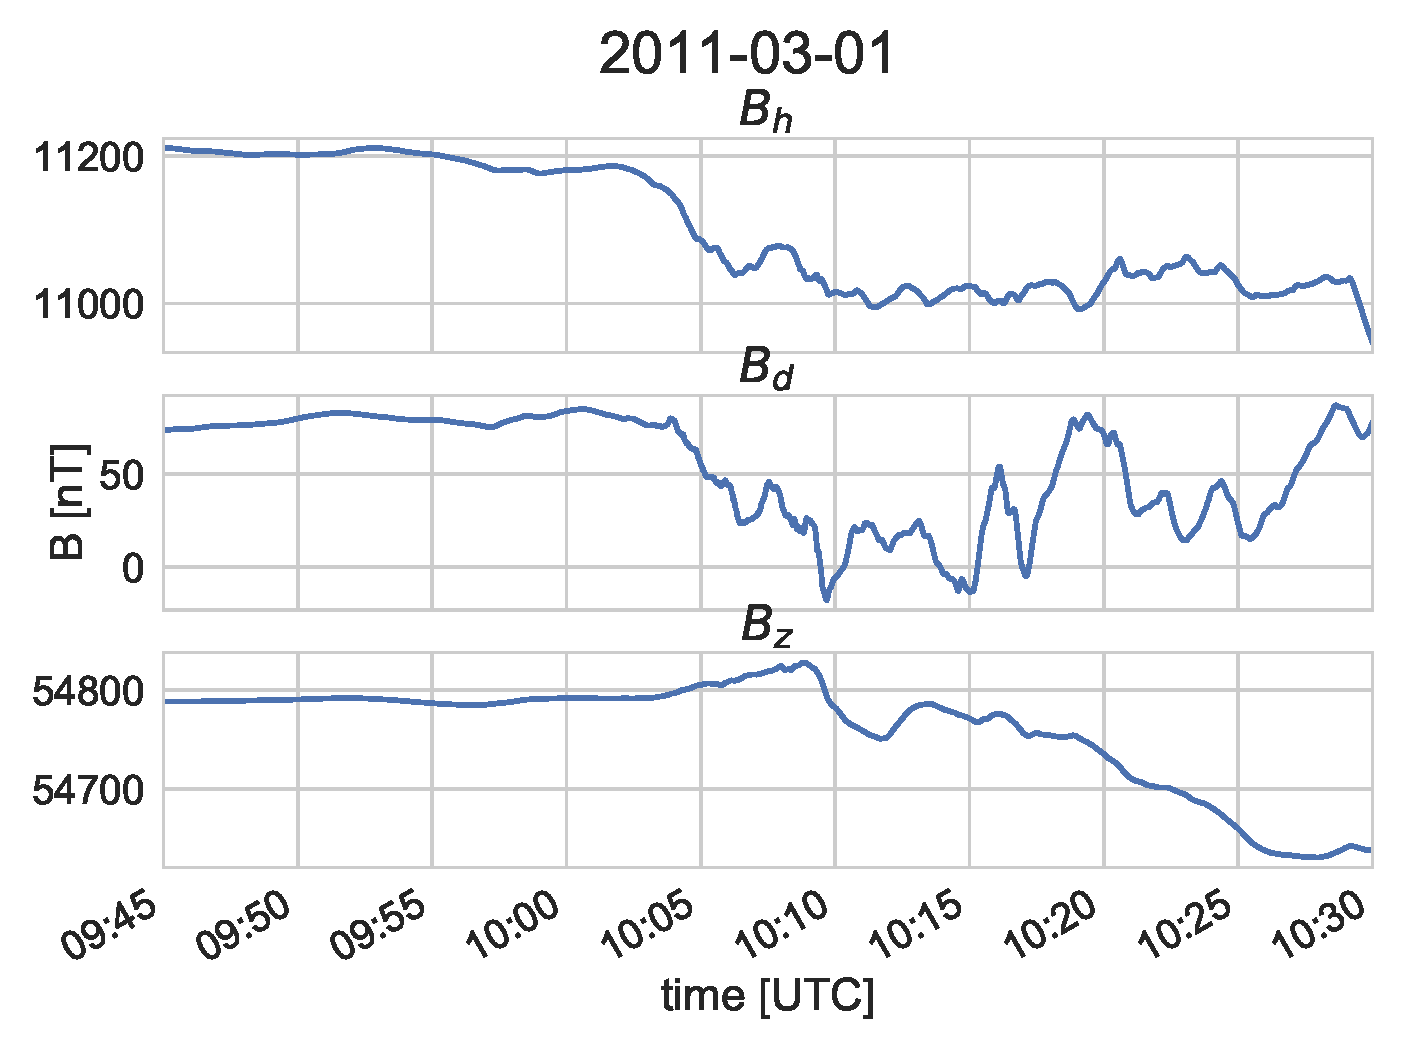
\includegraphics[width=\columnwidth]{gfx/2011-03-01/mag}
    \caption{Quiet conditions before the flaming auroral event are perturbed during the 2011-03-01 substorm.}
    \label{fig:mag20110301}
\end{figure}
The PF-DMSP spectrum of Figure~\ref{fig:msp20110301} had $I_{555.7}$ and $I_{427.8}$ available.
\begin{figure}\centering
    \includegraphics[width=\columnwidth]{gfx/2011-03-01/msp_ratio}
    \caption{PF-DMSP (a) $I_{555.7}$ and (b) $I_{427.8}$ with ratio (c) $I_{555.7} / I_{427.8}$. Around 10:06 and 10:11 UTC  intensifications near magnetic zenith indicates large increase in characteristic energy.}
    \label{fig:msp20110301}
\end{figure}
According to \citet{rees1974}, the magnetic zenith energies are on the order of \unit[5..10]{keV} during this event.
The PF-DMSP data is highly smeared in time across this event.
\citet{dahlgren2013} provided estimates using assumptions on the starting altitude of the flaming feature in a single-camera data inversion.
HiST was designed to study this type of event, with long-term automated recording so that events are not missed and the precipitation energy dynamics can be examined in more quantitative detail.

\FloatBarrier
\subsection{Kinked auroral arc}\label{sec:kink}
Auroral arcs with folds or kinks originate with magnetospheric configurations that are non-dispersive in nature.
Such disturbances also drive auroral vortices and vortex streets.
A striking example of a kinked auroral arc is shown in Figure~\ref{fig:20130414T0826}.
\begin{sidewaysfigure}\centering
    \noindent\includegraphics[width=\columnwidth,trim=15 697 25 0,clip]{gfx/2013-04-14T0826/2013-04-14T0826}

    \hspace{1.1cm}(a) 08:26:07.400 UT 
    \hspace{1.25cm}(b) 08:26:08.000 UT
    \hspace{1.1cm}(c) 08:26:08.100 UT
    \hspace{1.1cm}(d) 08:26:12.000 UT
    
    \caption{Narrow kinking and translating arcs at PFISR, ca. 08:26:10 UTC on April 14, 2013. 
          No coherent echoes detected in ion line, plasma line, or power spectral density.}
    %Two satellites cross through the field of view nearly orthogonally at 08:24:18 UTC.
    \label{fig:20130414T0826}
\end{sidewaysfigure}
A substorm is indicated as the initiator of the perturbation based on the southward turning IMF reflected in sharp negative excursion at 08:25 UTC as shown in Figure~\ref{fig:mag0826}.
\begin{figure}\centering
    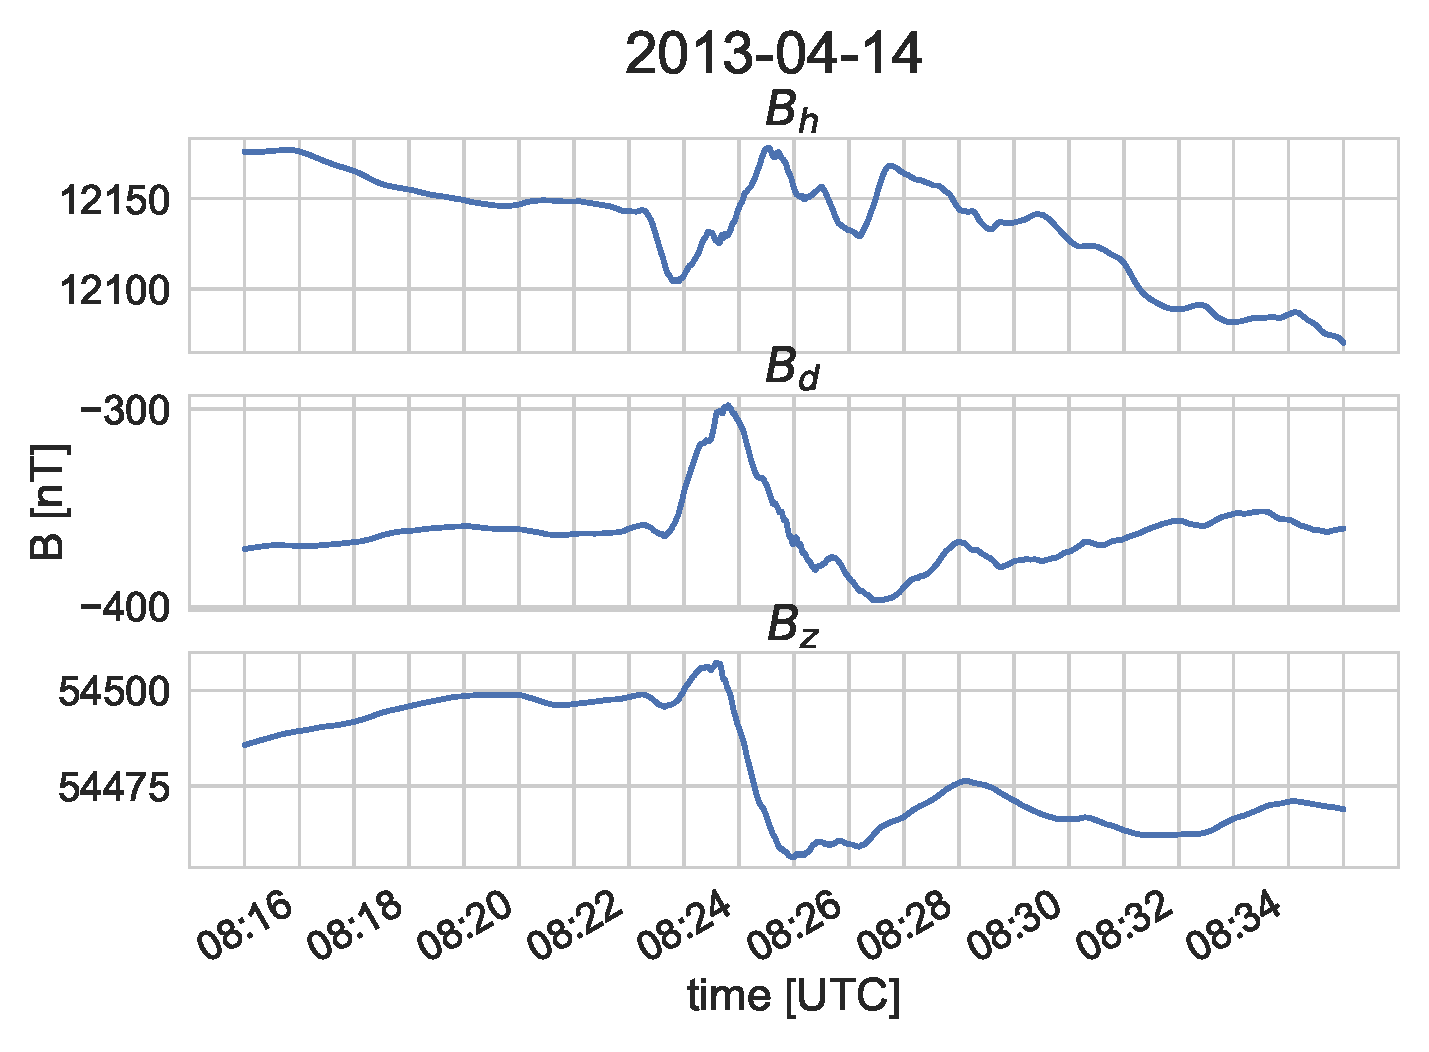
\includegraphics[width=\columnwidth]{gfx/2013-04-14T0826/mag}
    \caption{GIMA PFRR data showing geomagnetic field reversal near 08:25 UTC.}
    \label{fig:mag0826}
\end{figure}
A likely driver for this arc structure is an inverted-V acceleration region.
%As observed with HiST the auroral spectrum including the lines of Figure~\ref{fig:msp0826} is passed through the HiST BG3 filter, yielding $I_{557.7} \sim 0.01 \times I_{427.8}$.
The $I_{427.8}$ intensity suggests monoenergetic several keV electron beam configuration.
\begin{figure}
    \includegraphics[width=\columnwidth]{gfx/2013-04-14T0826/msp_spectra}
    \caption{PF-DMSP spectrum showing strong $I_{427.8}$, suggesting monoenergetic beam of several keV driving kinked arc near 08:26 UTC.}\label{fig:msp0826}
\end{figure}
Monoenergetic inverted-V accelerated electron differential number flux in the several keV range is the most likely candidate for generating this kinked aurora.